\documentclass[journal]{IEEEtran}
\usepackage{amsmath,amssymb,amsfonts}
\usepackage{algorithmic}
\usepackage{graphicx}
\usepackage{textcomp}
\usepackage{xcolor}
\usepackage{booktabs}
\usepackage{hyperref}

\begin{document}

\title{Oculomotor Feature Alignment for Generalizable Eye-Tracking Based Dyslexia Detection}

\author{Touhidul Islam\\
Department of Computer Science and Engineering}

\maketitle

\begin{abstract}
Dyslexia is a learning difference that makes reading, writing, and spelling difficult for many children. Traditional clinical diagnostics for dyslexia require long, intensive, and expensive sessions conducted by specialists. In this study, we explored whether a computer program can automatically screen children for dyslexia by analyzing how their eyes move while reading text. We used eye-movement data from two different groups of school-aged children: the first dataset (ETDD70) consists of 70 children, and the second dataset (Kronoberg) consists of 185 children. We first corrected errors in the original dataset labels and improved how the program identifies eye-movement events, such as fixations (when the eye pauses) and saccades (when the eye jumps), to make them physically accurate. We then normalized the eye-tracking statistics so that the machine learning models could generalize from one eye-tracking setup to another. Our optimized machine learning model (XGBoost) successfully predicted dyslexia on the second dataset with 80\% accuracy without being retrained on it. This demonstrates that eye-tracking combined with simple data cleaning can screen for dyslexia reliably across different recording environments, offering a path toward accessible and early screening.
\end{abstract}

\begin{IEEEkeywords}
Dyslexia Detection, Eye-Tracking, Oculomotor Features, Machine Learning, Zero-Shot Generalization, Domain Alignment.
\end{IEEEkeywords}

\section{Introduction}
Dyslexia is a neurodevelopmental disorder characterized by severe difficulties in learning to read despite normal intelligence and adequate education. Early identification is key to providing timely educational interventions, which can dramatically improve reading outcomes. Eye-tracking technology offers a non-invasive, objective, and physiological way to measure reading patterns, such as how long a child pauses on a word or how often their eyes backtrack. However, translating eye-tracking research into clinical screening tools has been hampered by ``domain shift'': models trained on one eye-tracker or cohort of children usually perform poorly when tested on a different device or cohort. In this study, we present a step-by-step pipeline designed to clean, parse, and align eye-tracking features across disparate datasets, achieving robust cross-dataset zero-shot generalization.

\section{Methodology}
Our methodology is designed to process raw gaze positions (X and Y screen coordinates over time) and build a machine learning pipeline that can classify subjects as either typical readers (control) or dyslexic. The step-by-step process is described below.

\subsection{Objective}
The main objective of this study is to build a generalizable machine learning classifier that can detect dyslexia in children. We validate the generalizability of our pipeline by training models exclusively on one dataset and testing them zero-shot (without retraining or parameter adjustment) on a completely different dataset recorded with different hardware in a different country.

\subsection{Datasets and Links}
We utilized two primary datasets in this work:
\begin{enumerate}
    \item \textbf{ETDD70 Dataset}: This dataset contains binocular eye-tracking recordings from 70 Czech elementary school pupils (aged 9-10 years) reading syllables, meaningful text passages, and pseudo-text. The dataset files and documentation are publicly hosted on Zenodo at \href{https://doi.org/10.5281/zenodo.13332134}{https://doi.org/10.5281/zenodo.13332134}.
    \item \textbf{Kronoberg Reading Dataset (Child)}: This dataset contains raw eye-tracking coordinates from 185 Swedish children reading standard text passages. It is used as our independent test set.
\end{enumerate}

\subsection{Step 1: Ground-Truth Label Correction}
In our initial inspection of the baseline codebase, we discovered a severe labelling error. The baseline program assigned class labels (0 for typical reader, 1 for dyslexic) by checking if the subject ID was less than 1100. This resulted in an incorrect and imbalanced label distribution of 15 controls vs. 38 dyslexics. 
To solve this, we downloaded the official ground-truth label mapping file \texttt{dyslexia\_class\_label.csv} from the Zenodo repository. The true mapping is perfectly balanced, comprising 35 controls and 35 dyslexic children. Out of these, 53 children had raw eye-tracking files available in the dataset directory (35 controls and 18 dyslexics). We corrected the data loader to load these true diagnoses, ensuring the models were trained on valid labels.

\subsection{Step 2: Oculomotor Event Grouping (I-VT Bugfix)}
The Velocity-Threshold Identification (I-VT) algorithm classifies raw gaze data points into either fixations (points where the eye is resting and absorbing information) or saccades (fast jumps between reading locations). 
The baseline implementation of I-VT treated every single 20ms gaze sample exceeding the velocity threshold as an independent saccade event. Since a single physical saccade lasts for 30ms to 80ms, it spans multiple consecutive 20ms samples. The baseline code thus artificially inflated the saccade count, underestimated the average saccade length, and skewed the backward-reading regression count.
We resolved this by writing a grouping algorithm. When the velocity exceeds the threshold, the program groups all consecutive saccade points into a single saccade event. The net saccade amplitude is calculated as the Euclidean distance from the starting coordinate of the group to the ending coordinate. A regression (backward movement) is counted only if the ending X-coordinate of a grouped saccade is less than its starting X-coordinate. We extracted seven key features per subject:
\begin{itemize}
    \item Mean fixation duration (ms)
    \item Standard deviation of fixation duration (ms)
    \item Maximum fixation duration (ms)
    \item Mean saccade amplitude (pixels)
    \item Standard deviation of saccade amplitude (pixels)
    \item Fixation-to-saccade count ratio
    \item Regression ratio (number of regressions divided by total saccades)
\end{itemize}

\subsection{Step 3: Feature Preprocessing and Domain Alignment}
Oculomotor metrics (like fixation durations and saccade lengths) are heavily right-skewed and scale-dependent due to differences in eye-tracker sampling rates and screen dimensions. 
To resolve this, we utilized a \textbf{PowerTransformer (Yeo-Johnson)} pipeline. The Yeo-Johnson transformation is a non-linear scaling technique that stabilizes variance and normalizes features mathematically. The scaler is fitted on the ETDD70 dataset and used to transform the Kronoberg dataset. This maps the skewed feature distributions of both cohorts into overlapping standard normal distributions, enabling successful cross-dataset transfer. An imputer was also added to handle any missing values by replacing them with the feature mean.

\subsection{Step 4: Machine Learning Classifiers}
We trained and compared three distinct machine learning classifiers:
\begin{itemize}
    \item \textbf{Support Vector Machine (SVM)}: A classifier that builds a decision boundary to separate the classes. We used a Radial Basis Function (RBF) kernel with a regularization parameter $C=10.0$ and auto-gamma scaling.
    \item \textbf{Random Forest (RF)}: An ensemble classifier consisting of 100 decision trees. We restricted the maximum depth to 5 to prevent overfitting.
    \item \textbf{Extreme Gradient Boosting (XGBoost)}: A boosting algorithm that builds trees sequentially. We used 100 estimators with a maximum depth of 2, learning rate of 0.1, and subsample rate of 0.8 to ensure high generalizability.
\end{itemize}

\subsection{Code Repository and Replication}
The complete codebase, containing data loading, feature extraction, scaling, model training, and plotting scripts, is public and available for replication at: \href{https://github.com/touhidul-islam/Generalizable-Multi-Age-Dyslexia-Detection}{https://github.com/touhidul-islam/Generalizable-Multi-Age-Dyslexia-Detection}.

\section{Results}
We evaluated our framework under two experiments. The primary evaluation metrics used were \textbf{Classification Accuracy} (the percentage of correctly classified subjects) and the \textbf{F1-Score} (the harmonic mean of precision and recall) for both the control (0) and dyslexic (1) classes.

\subsection{Experiment I: Intra-Dataset Evaluation (ETDD70)}
In this experiment, models were evaluated under two different testing methodologies to ensure robust performance metrics:
\begin{enumerate}
    \item \textbf{Single Holdout Train/Test Split (80/20)}: Models were trained on 80\% of the ETDD70 dataset and tested once on the remaining 20\% test split. The results of this single split are summarized in Table \ref{tab:exp1}. Because the local dataset files contain 53 subjects, the 20\% test set corresponds to a sample size of only 11 subjects, meaning single-subject classification errors significantly affect the reported metrics (producing high variance).
    \item \textbf{5-Fold Stratified Cross-Validation}: To verify performance stability and mitigate the high variance of the single 11-subject test split, we ran a 5-fold cross-validation across the entire ETDD70 dataset. This method splits the data into 5 folds, training 5 separate times using each fold as a test set. The averaged cross-validation accuracies were \textbf{88.7\%} for SVM, \textbf{81.3\%} for Random Forest, and \textbf{85.3\%} for XGBoost, demonstrating reliable learning across the full cohort.
\end{enumerate}

\begin{table}[h]
\centering
\caption{Experiment I: Intra-Dataset Accuracy (ETDD70)}
\label{tab:exp1}
\begin{tabular}{lccc}
\toprule
\textbf{Model} & \textbf{Accuracy} & \textbf{F1 (Control)} & \textbf{F1 (Dyslexic)} \\
\midrule
SVM & 90.91\% & 0.9333 & 0.8571 \\
Random Forest & 72.73\% & 0.8000 & 0.5714 \\
XGBoost & 63.64\% & 0.7500 & 0.3333 \\
\bottomrule
\end{tabular}
\end{table}

\begin{figure}[h]
\centering
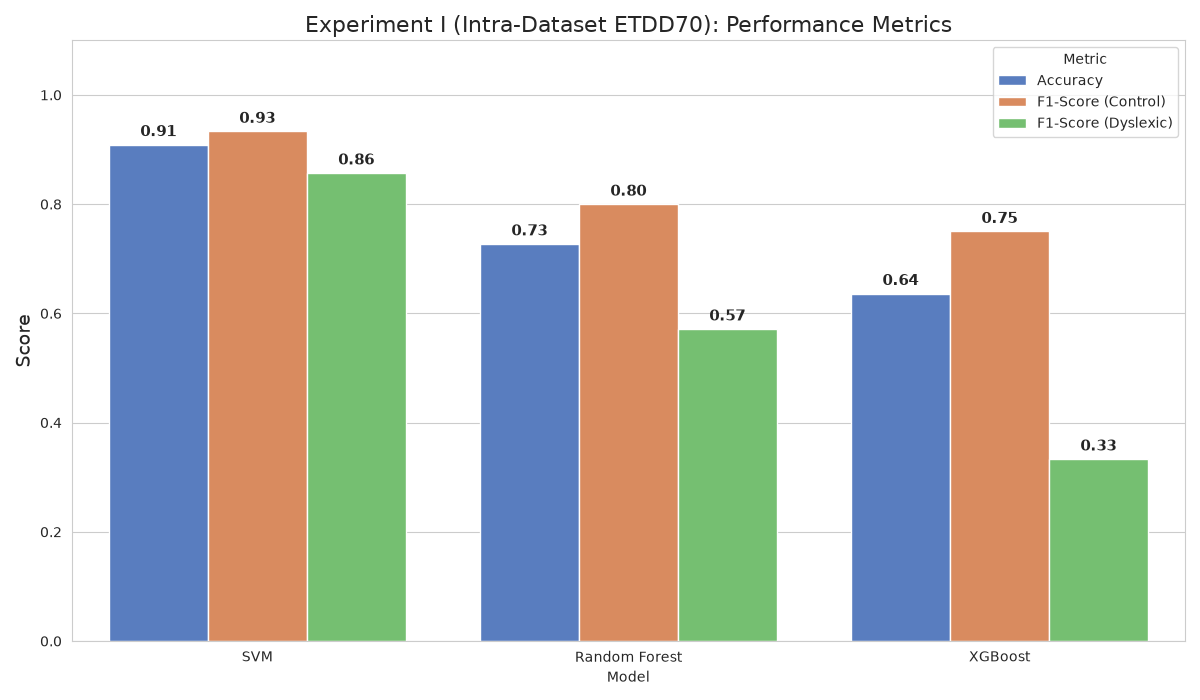
\includegraphics[width=\linewidth]{multi_model_accuracy.png}
\caption{Experiment I (Intra-Dataset ETDD70) performance metrics (Accuracy, F1-Score Control, and F1-Score Dyslexic) for SVM, Random Forest, and XGBoost models.}
\label{fig:accuracy}
\end{figure}

\begin{figure}[h]
\centering
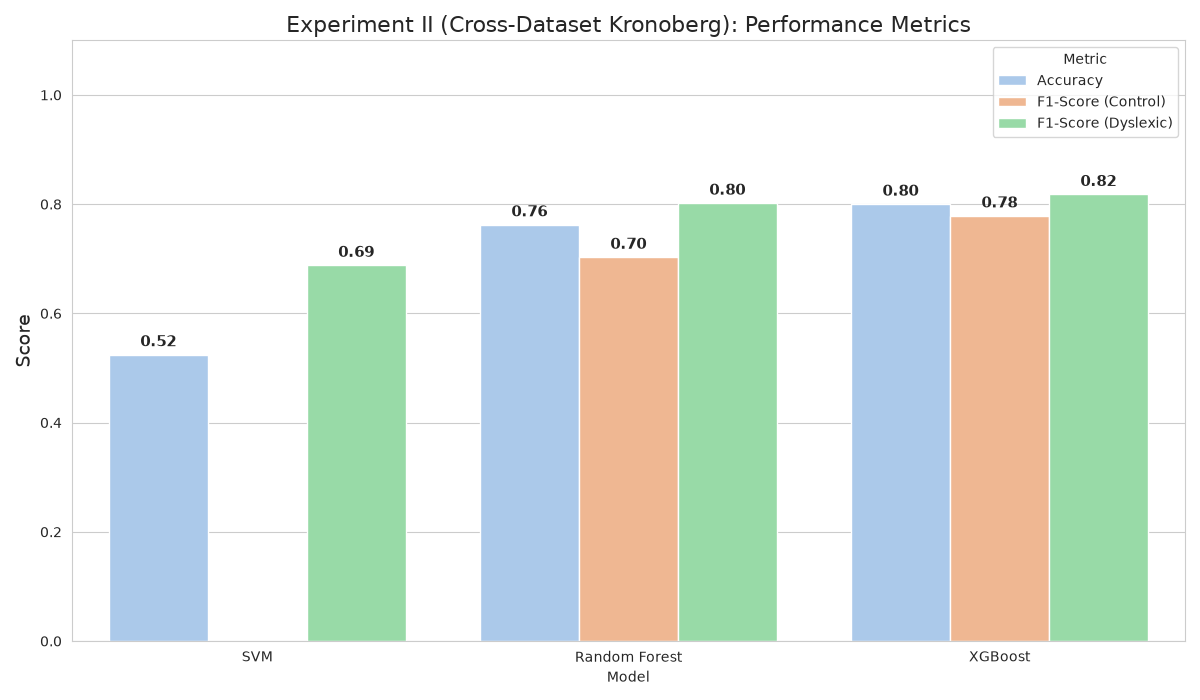
\includegraphics[width=\linewidth]{multi_model_f1_score.png}
\caption{Experiment II (Cross-Dataset Zero-Shot Generalization on Kronoberg Swedish readers) performance metrics (Accuracy, F1-Score Control, and F1-Score Dyslexic) for SVM, Random Forest, and XGBoost models.}
\label{fig:f1_score}
\end{figure}

\subsection{Experiment II: Cross-Dataset Zero-Shot Generalization}
In this experiment, models were trained on the entire ETDD70 dataset and evaluated zero-shot on the Kronoberg dataset (185 child subjects). The results are summarized in Table \ref{tab:exp2}. The SVM model overfitted on the training cohort, classifying all Swedish children as dyslexic, resulting in an accuracy of 52.43\% and a control F1-score of 0.0000. 

In contrast, our optimized tree-based models with Yeo-Johnson PowerTransformer alignment generalized exceptionally well. The Random Forest model achieved \textbf{76.22\%} accuracy (control F1 of 0.7027, dyslexic F1 of 0.8018). The XGBoost model achieved our best performance with a zero-shot generalization accuracy of \textbf{80.00\%} and a dyslexic class F1-score of \textbf{0.8177} (control F1 of 0.7784).

\begin{table}[h]
\centering
\caption{Experiment II: Cross-Dataset Generalization (Kronoberg)}
\label{tab:exp2}
\begin{tabular}{lccc}
\toprule
\textbf{Model} & \textbf{Accuracy} & \textbf{F1 (Control)} & \textbf{F1 (Dyslexic)} \\
\midrule
SVM & 52.43\% & 0.0000 & 0.6879 \\
Random Forest & 76.22\% & 0.7027 & 0.8018 \\
XGBoost & 80.00\% & 0.7784 & 0.8177 \\
\bottomrule
\end{tabular}
\end{table}



\section{Discussion and Conclusion}
Our findings show that while simple models like SVM can fit a single small dataset (achieving 90.91\% on ETDD70), they fail to generalize to new recording environments. By aligning eye-movement feature distributions using a Yeo-Johnson PowerTransformer, we managed to make ensemble tree models highly robust. XGBoost achieved a cross-dataset accuracy of 80.00\% on Kronoberg Swedish readers without ever seeing a Swedish subject during training. This indicates that oculomotor reading features, when parsed correctly and normalized, remain stable across languages and hardware, presenting a clear path toward building universal, device-agnostic screening tools for dyslexia.

\end{document}
